\documentclass{ecai2014}
\usepackage{times}
\usepackage{graphicx}
\usepackage{latexsym}
\usepackage{url}
\usepackage{subfig}
\usepackage{amsbsy}

%\ecaisubmission   % inserts page numbers. Use only for submission of paper.
                  % Do NOT use for camera-ready version of paper.

\begin{document}

\title{Local Image Descriptor Inspired by Visual Cortex}

\author{Hui Wei \and Zheng Dong\institute{
Department of Computer Science, 
Laboratory of Cognitive Model and Algorithm,
Shanghai Key Laboratory of Data Science, 
Fudan University, China, email: weihui@fudan.edu.cn} }

\maketitle
\bibliographystyle{ecai2014}

\begin{abstract}
The ability of visual cortex to accomplish object recognition
tasks accurately and effortlessly makes it an attractive
goal of computer vision to emulate the mechanism of the cortex. 
The neural process of object recognition in the brain follows a hierarchical scheme.
In this paper, we present a novel model inspired by the visual pathway in primate brains.
This multi-layer neural network model imitates
the hierarchical convergent processing mechanism of the visual pathway.
We show experimentally that local image features generated by this model exhibit robust discrimination 
and even better generalization ability compared with some existing image descriptors.
We also demonstrate the application of this model to object recognition tasks. 
The result provides strong support for the potential of this model.
\end{abstract}

\section{INTRODUCTION}

In this paper, we propose a multi-layer neural network model which imitates the neural mechanism
of the ventral visual pathway \cite{Lehky2007}, which is involved in object recognition.
The ventral pathway travels through V1 and some other visual areas (V2 and V4) 
and finally reaches the inferior temporal (IT) cortex.
In our model, different stages of the pathway are explicitly mapped 
to different layers of a feed-forward neural network.
With this network, high-level local image features are extracted from images.
These features exhibit competitive performance when applied to computer vision tasks.

\section{MULTI-LAYER NEURAL NETWORK}\label{sec:model}

Four stages in the ventral pathway are mapped to four layers in our neural network.
They are composed of simple cells, complex cells, V4 neurons and IT neurons respectively 
(\figurename~\ref{fig:model}). 

\begin{figure}[h]
\centering
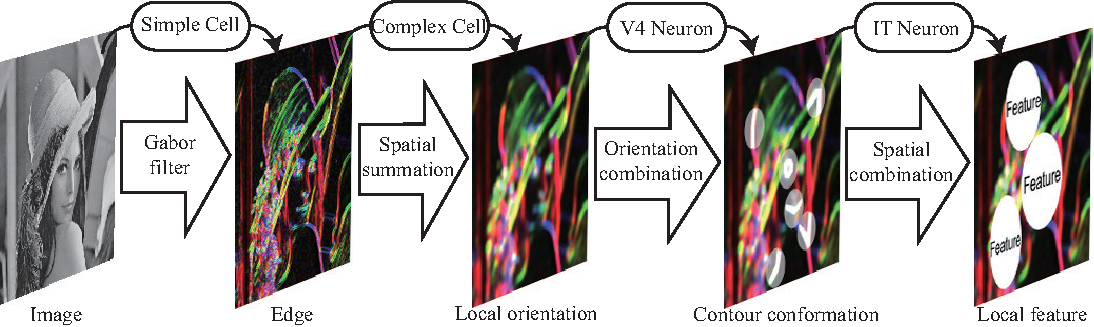
\includegraphics[width=0.98\linewidth]{images/fig1.pdf}
\caption{Multilayer neural network inspired by ventral pathway.}
\label{fig:model}
\end{figure}


Simple cells \cite{Hubel1962} respond primarily to oriented edges and gratings.
They can be understood as linear filters modeled as Gabor functions \cite{Gabor1946}
like equation \ref{equ:gabor},
where $x'=x\cos\theta+y\sin\theta$, $y'=-x\sin\theta+y\cos\theta$.
In the equation, $\lambda$ is the wavelength of the sinusoidal factor, 
$\theta$ represents the preferred orientation and 
$\sigma_s$ approximates the radius of the receptive fields.

\begin{equation}\label{equ:gabor}
g_{\theta}(x,y;\lambda,\sigma_s)
=\exp\left(-\frac{x'^2+y'^2}{2\sigma_s^2}\right)
\cos(2\pi x'/\lambda),
\end{equation}

Complex cells differ from simple cells in that a stimulus is effective wherever it is placed 
in the receptive field, provided that the orientation is appropriate \cite{Hubel1962}. 
In our model, complex cells are modeled as weighted summation of the absolute value of simple cell output.
The weight function is Gaussian function, 
$f(x,y;\sigma_c)=\frac{1}{2\pi\sigma_c^2}\exp\left(-\frac{x^2+y^2}{2\sigma_c^2}\right)$,
where $\sigma_c=2\sigma_s$ represents the radius of the complex receptive fields.
Given $I(x,y)$ as some input image, 
the output of complex cells
with the preferred orientation $\theta$
is calculated as the following convolution,
\begin{equation}
C_{\theta}=|I\otimes g_{\theta}|\otimes f.
\label{equ:complex}
\end{equation}

V4 neurons are selectively tuned for curvature and angular position of convex boundaries \cite{Pasupathy2001}.
In the experiment demonstrated in \figurename~\ref{fig:v4it}a and \ref{fig:v4it}b,
a single-layer perceptron which takes complex cells as input is trained
to selectively respond to a sharp convex angle towards the top-right \cite{Pasupathy2001}.
This experiment shows that complex cells provide sufficient information for the emergence of V4 selectivity.
Therefore V4 neurons in our model combine the output of complex cells that share the same receptive field.
The V4 output at a given position $(x,y)$ is a vector defined as follows.
\begin{equation}
\boldsymbol{\vec{V}}(x,y) = \sum_{k} C_{\theta_k}(x,y) \cdot \boldsymbol{\vec{e}}_k,
\label{equ:v4}
\end{equation}
where $\{\boldsymbol{\vec{e}}_k:k=1,2,3,\cdots\}$ is a group of standard basis;
$C_{\theta_k}$ is the output of complex cells with preferred orientation $\theta_k$ defined by equation (\ref{equ:complex}).

\begin{figure}[h]
\centering
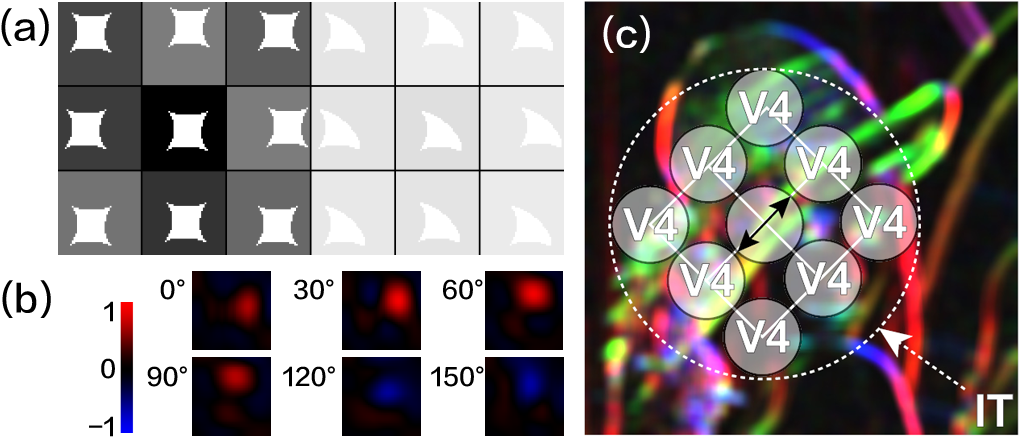
\includegraphics[width=0.75\linewidth]{images/fig2.png}
\caption{V4 and IT. 
(a) V4 perceptron was trained to distinguish a sharp convex angle towards the top-right.
The gray scale of the background indicates the strength of response.
(b) The weight matrix of the V4 perceptron. Each block corresponds to a specific orientation.
(c) V4 neurons in 9 grid points contribute to an IT neuron.
The grid is rotated to the major orientation of the central V4 unit.}
\label{fig:v4it}
\end{figure}

The IT neuron collects the responses from a group of afferent V4 neurons 
and synthesizes a unified representation of shapes.
In our model, the IT output is a vector produced by concatenating the output vectors of V4 neurons.
We choose afferent V4 neurons from $3\times 3$ rectangular grid points (\figurename~\ref{fig:v4it}c).
The gird is rotated to the strongest orientation of the central V4 input 
in order to achieve the invariance of feature orientations.

\section{EMPIRICAL EVALUATION}\label{sec:exp}

We demonstrate the performance of the features generated by our model 
in feature matching and object recognition tasks.

We provide a qualitative evaluation of our features by matching features between different images.
The SIFT features are used for comparison.
The VLFeat library \cite{Vedaldi2008} were utilized for the SIFT implementation and the feature matching algorithm.

\begin{figure}[h]
\centering
  \subfloat[Matching between the same face]{
    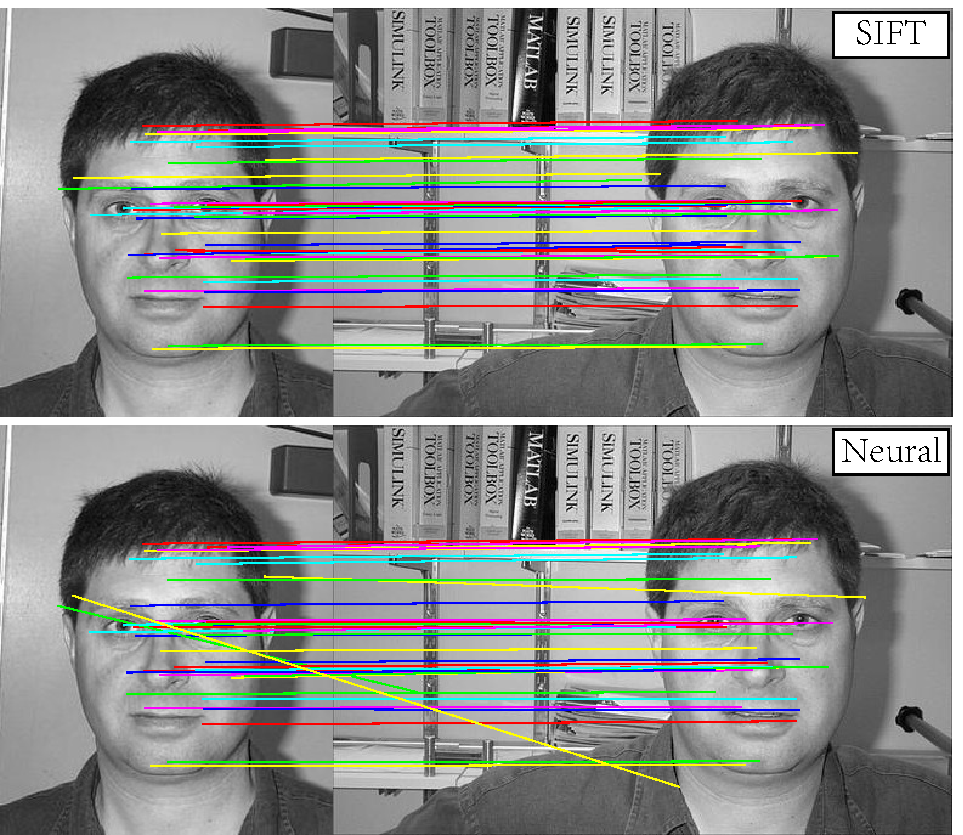
\includegraphics[width=0.5\linewidth]{images/fig4a.pdf}
    \label{fig:face:same}}
  \subfloat[Matching between different faces]{
    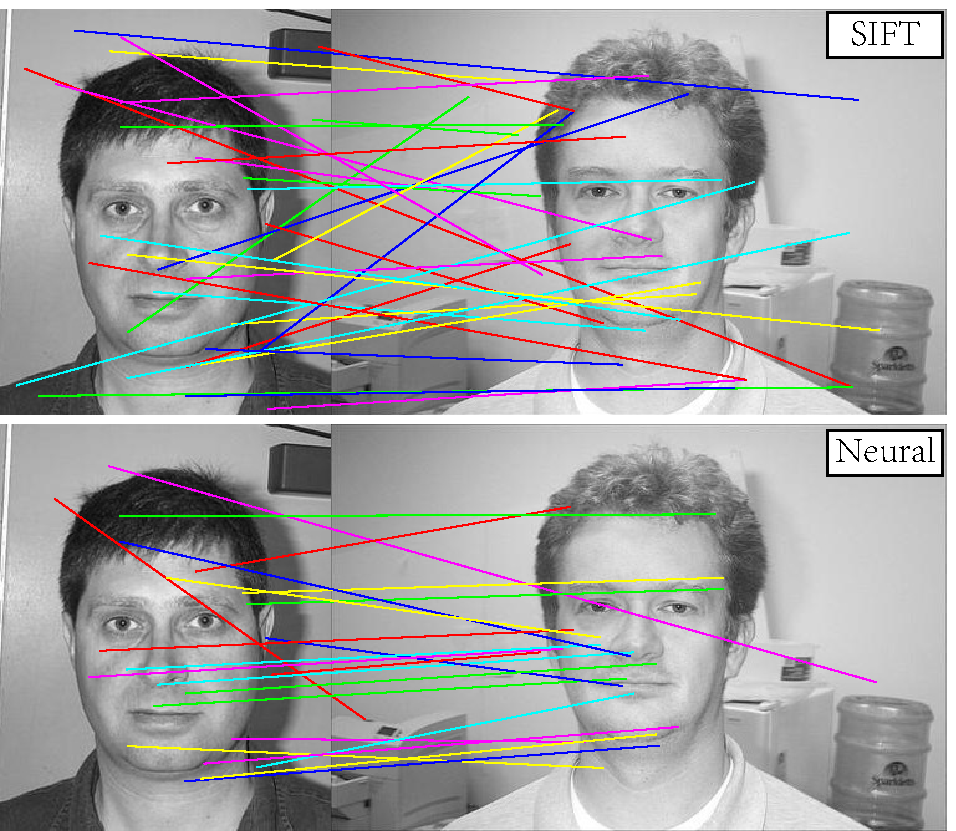
\includegraphics[width=0.5\linewidth]{images/fig4b.pdf}
    \label{fig:face:diff}}
\caption{Matching face images.}
\label{fig:facematch}
\end{figure}

As shown in \figurename~\ref{fig:face:same}, SIFT features match perfectly between face images of the same person.
The neural features generated by our model achieve competitive distinctiveness.
However, \figurename~\ref{fig:face:diff} shows that 
matching of SIFT features between face images of different people is quite disordered.
SIFT features excel in matching highly distinctive features under image transformations 
but lack the generalization ability to capture variations in objects appearance of the same category.
By contrast, the neural features show robust performance in matching features from different faces.
The result suggests that our model exhibits better generalization ability.

We also evaluate the performance of the proposed model in object recognition tasks
with the Caltech 101 dataset \cite{Fei-Fei2004}.
We use the bag of words approach for object recognition.
Key-points are detected with the salient region detector proposed by Kadir and Brady \cite{Kadir2001}.
Features at the key-points are extracted with our model and passed to an SVM classifier.
We investigate the selection of sampling density of preferred orientations,
i.e., how many orientations a V4 output vector contains.
The result averaged over 8 independent runs is shown in \figurename~\ref{fig:result:density}.
As is shown, the selection of sampling density does not exhibit obvious impact on the performance.
In the succeeding experiments, a sampling density of $3$ is used. 
To investigate the contribution of the number of features on performance,
we vary the number of features chosen from each training image.
The result shown in \figurename~\ref{fig:result:nfeature} is also averaged over 8 independent runs.
With 50 features per image the result approaches the best performance.
In the succeeding experiments, 50 features are extracted from each image.

\begin{figure}[h]
\centering
  \subfloat[Sampling density of orientations]{
    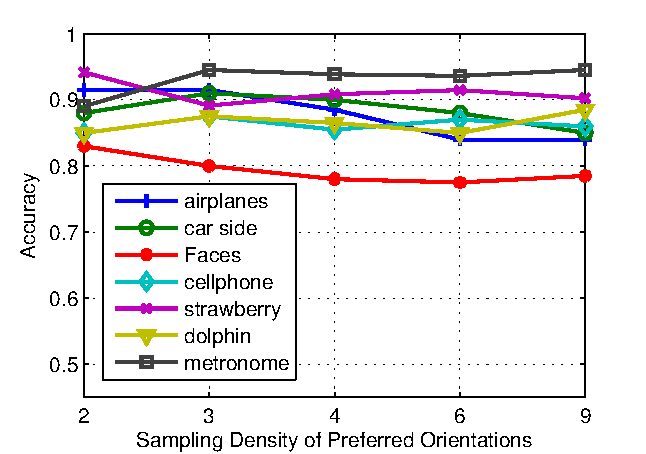
\includegraphics[width=0.5\linewidth]{images/fig5a.pdf}
    \label{fig:result:density}}
  \subfloat[Number of features per image]{
    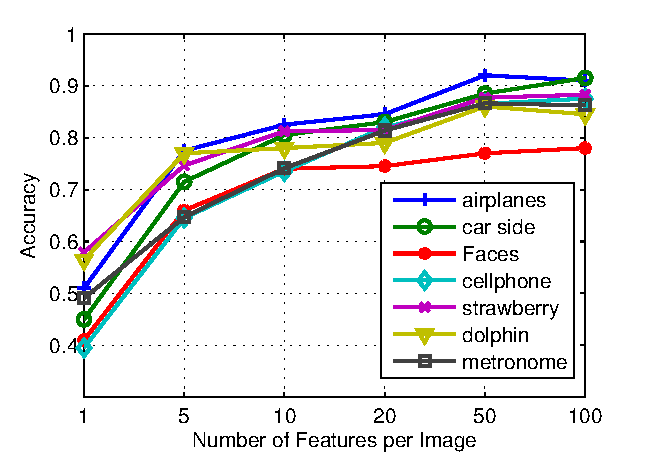
\includegraphics[width=0.5\linewidth]{images/fig5b.pdf}
    \label{fig:result:nfeature}}\\
  \subfloat[Comparison with other methods]{
    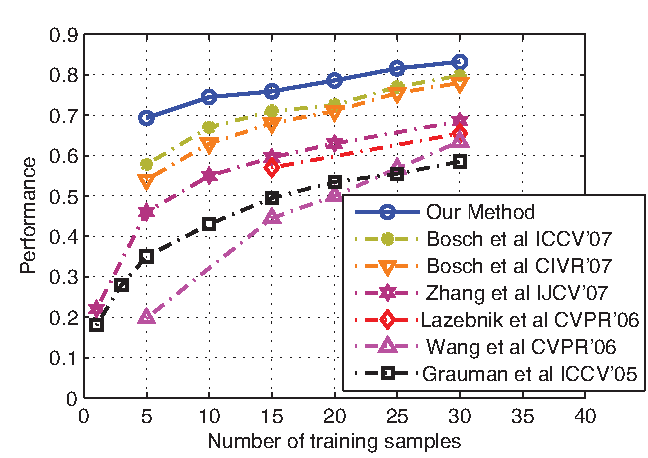
\includegraphics[width=0.5\linewidth]{images/fig5c.pdf}
    \label{fig:result:ntrain}}
  \subfloat[Comparison with other features]{
    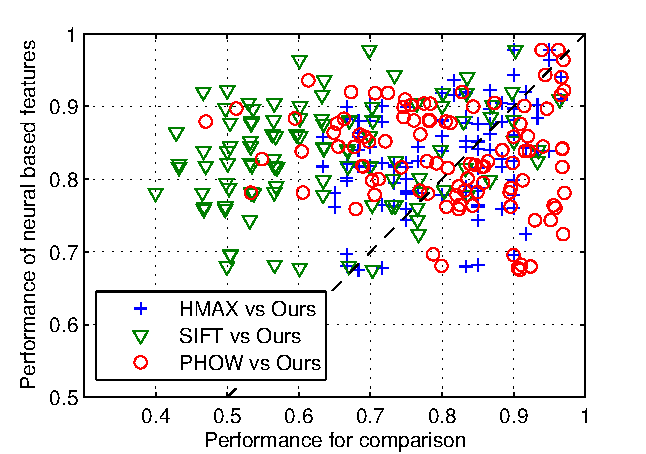
\includegraphics[width=0.5\linewidth]{images/fig5d.pdf}
    \label{fig:result:compare}}
\caption{Performance with different parameters.}
\label{fig:result}
\end{figure}

The performance of our model is compared with published result
in \figurename~\ref{fig:result:ntrain}.
The performance is averaged over all categories and
the comparison was taken over different number of training images.
\figurename~\ref{fig:result:compare} shows
the performance of our model over the 101 categories
compared with SIFT features \cite{Lowe1999},
PHOW features \cite{Lazebnik2006},
and biologically inspired HMAX model \cite{Serre2007}.
The results are obtained with 30 training images randomly selected from each category.
Our model exhibits competitive performance compared with other models.

\ack This work was supported by the 973 Program (Project No. 2010CB327900), 
the NSFC project (Project No. 61375122, 81373556), 
and the National ``Twelfth Five-Year Plan'' for Science and Technology (Project No. 2012BAI37B06).

\bibliography{ecai2014}
\end{document}
%%%%%%%%%%%%%%%%%%%%%%%%%%%%%%%%%%%%%%%%%%%%%%%%%%%%%%%%%%%%%%%%%%%%%%
